% This file was created with tikzplotlib v0.10.1.
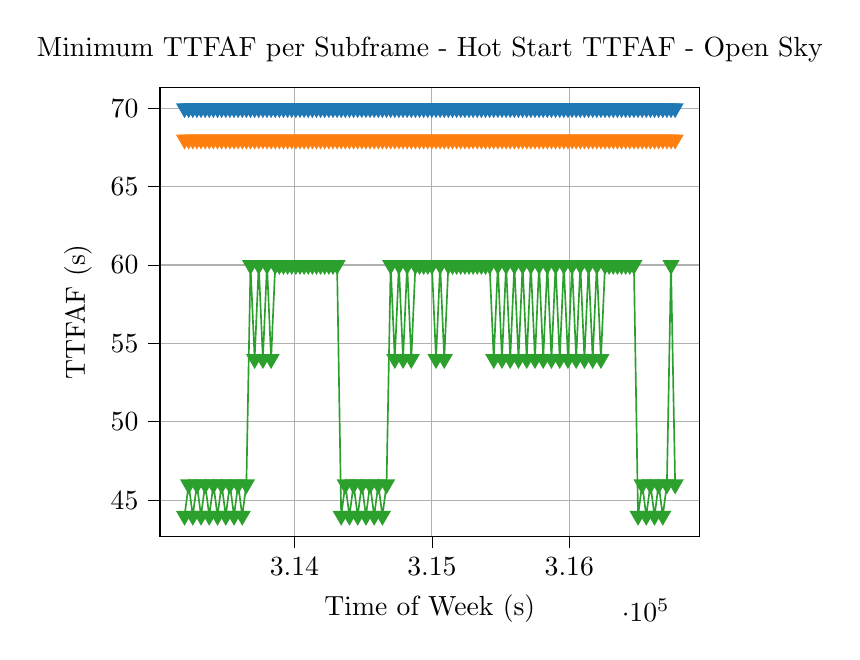
\begin{tikzpicture}

\definecolor{darkgray176}{RGB}{176,176,176}
\definecolor{darkorange25512714}{RGB}{255,127,14}
\definecolor{forestgreen4416044}{RGB}{44,160,44}
\definecolor{steelblue31119180}{RGB}{31,119,180}

\begin{axis}[
tick align=outside,
tick pos=left,
title={Minimum TTFAF per Subframe - Hot Start TTFAF - Open Sky},
x grid style={darkgray176},
xlabel={Time of Week (s)},
xmajorgrids,
xmin=313021.5, xmax=316948.5,
xtick style={color=black},
y grid style={darkgray176},
ylabel={TTFAF (s)},
ymajorgrids,
ymin=42.7, ymax=71.3,
ytick style={color=black}
]
\addplot [semithick, steelblue31119180, mark=triangle*, mark size=3, mark options={solid,rotate=180}, only marks]
table {%
313200 70
313230 70
313260 70
313290 70
313320 70
313350 70
313380 70
313410 70
313440 70
313470 70
313500 70
313530 70
313560 70
313590 70
313620 70
313650 70
313680 70
313710 70
313740 70
313770 70
313800 70
313830 70
313860 70
313890 70
313920 70
313950 70
313980 70
314010 70
314040 70
314070 70
314100 70
314130 70
314160 70
314190 70
314220 70
314250 70
314280 70
314310 70
314340 70
314370 70
314400 70
314430 70
314460 70
314490 70
314520 70
314550 70
314580 70
314610 70
314640 70
314670 70
314700 70
314730 70
314760 70
314790 70
314820 70
314850 70
314880 70
314910 70
314940 70
314970 70
315000 70
315030 70
315060 70
315090 70
315120 70
315150 70
315180 70
315210 70
315240 70
315270 70
315300 70
315330 70
315360 70
315390 70
315420 70
315450 70
315480 70
315510 70
315540 70
315570 70
315600 70
315630 70
315660 70
315690 70
315720 70
315750 70
315780 70
315810 70
315840 70
315870 70
315900 70
315930 70
315960 70
315990 70
316020 70
316050 70
316080 70
316110 70
316140 70
316170 70
316200 70
316230 70
316260 70
316290 70
316320 70
316350 70
316380 70
316410 70
316440 70
316470 70
316500 70
316530 70
316560 70
316590 70
316620 70
316650 70
316680 70
316710 70
316740 70
316770 70
};
\addplot [semithick, steelblue31119180]
table {%
313200 70
313230 70
313260 70
313290 70
313320 70
313350 70
313380 70
313410 70
313440 70
313470 70
313500 70
313530 70
313560 70
313590 70
313620 70
313650 70
313680 70
313710 70
313740 70
313770 70
313800 70
313830 70
313860 70
313890 70
313920 70
313950 70
313980 70
314010 70
314040 70
314070 70
314100 70
314130 70
314160 70
314190 70
314220 70
314250 70
314280 70
314310 70
314340 70
314370 70
314400 70
314430 70
314460 70
314490 70
314520 70
314550 70
314580 70
314610 70
314640 70
314670 70
314700 70
314730 70
314760 70
314790 70
314820 70
314850 70
314880 70
314910 70
314940 70
314970 70
315000 70
315030 70
315060 70
315090 70
315120 70
315150 70
315180 70
315210 70
315240 70
315270 70
315300 70
315330 70
315360 70
315390 70
315420 70
315450 70
315480 70
315510 70
315540 70
315570 70
315600 70
315630 70
315660 70
315690 70
315720 70
315750 70
315780 70
315810 70
315840 70
315870 70
315900 70
315930 70
315960 70
315990 70
316020 70
316050 70
316080 70
316110 70
316140 70
316170 70
316200 70
316230 70
316260 70
316290 70
316320 70
316350 70
316380 70
316410 70
316440 70
316470 70
316500 70
316530 70
316560 70
316590 70
316620 70
316650 70
316680 70
316710 70
316740 70
316770 70
};
\addplot [semithick, darkorange25512714, mark=triangle*, mark size=3, mark options={solid,rotate=180}, only marks]
table {%
313200 68
313230 68
313260 68
313290 68
313320 68
313350 68
313380 68
313410 68
313440 68
313470 68
313500 68
313530 68
313560 68
313590 68
313620 68
313650 68
313680 68
313710 68
313740 68
313770 68
313800 68
313830 68
313860 68
313890 68
313920 68
313950 68
313980 68
314010 68
314040 68
314070 68
314100 68
314130 68
314160 68
314190 68
314220 68
314250 68
314280 68
314310 68
314340 68
314370 68
314400 68
314430 68
314460 68
314490 68
314520 68
314550 68
314580 68
314610 68
314640 68
314670 68
314700 68
314730 68
314760 68
314790 68
314820 68
314850 68
314880 68
314910 68
314940 68
314970 68
315000 68
315030 68
315060 68
315090 68
315120 68
315150 68
315180 68
315210 68
315240 68
315270 68
315300 68
315330 68
315360 68
315390 68
315420 68
315450 68
315480 68
315510 68
315540 68
315570 68
315600 68
315630 68
315660 68
315690 68
315720 68
315750 68
315780 68
315810 68
315840 68
315870 68
315900 68
315930 68
315960 68
315990 68
316020 68
316050 68
316080 68
316110 68
316140 68
316170 68
316200 68
316230 68
316260 68
316290 68
316320 68
316350 68
316380 68
316410 68
316440 68
316470 68
316500 68
316530 68
316560 68
316590 68
316620 68
316650 68
316680 68
316710 68
316740 68
316770 68
};
\addplot [semithick, darkorange25512714]
table {%
313200 68
313230 68
313260 68
313290 68
313320 68
313350 68
313380 68
313410 68
313440 68
313470 68
313500 68
313530 68
313560 68
313590 68
313620 68
313650 68
313680 68
313710 68
313740 68
313770 68
313800 68
313830 68
313860 68
313890 68
313920 68
313950 68
313980 68
314010 68
314040 68
314070 68
314100 68
314130 68
314160 68
314190 68
314220 68
314250 68
314280 68
314310 68
314340 68
314370 68
314400 68
314430 68
314460 68
314490 68
314520 68
314550 68
314580 68
314610 68
314640 68
314670 68
314700 68
314730 68
314760 68
314790 68
314820 68
314850 68
314880 68
314910 68
314940 68
314970 68
315000 68
315030 68
315060 68
315090 68
315120 68
315150 68
315180 68
315210 68
315240 68
315270 68
315300 68
315330 68
315360 68
315390 68
315420 68
315450 68
315480 68
315510 68
315540 68
315570 68
315600 68
315630 68
315660 68
315690 68
315720 68
315750 68
315780 68
315810 68
315840 68
315870 68
315900 68
315930 68
315960 68
315990 68
316020 68
316050 68
316080 68
316110 68
316140 68
316170 68
316200 68
316230 68
316260 68
316290 68
316320 68
316350 68
316380 68
316410 68
316440 68
316470 68
316500 68
316530 68
316560 68
316590 68
316620 68
316650 68
316680 68
316710 68
316740 68
316770 68
};
\addplot [semithick, forestgreen4416044, mark=triangle*, mark size=3, mark options={solid,rotate=180}, only marks]
table {%
313200 44
313230 46
313260 44
313290 46
313320 44
313350 46
313380 44
313410 46
313440 44
313470 46
313500 44
313530 46
313560 44
313590 46
313620 44
313650 46
313680 60
313710 54
313740 60
313770 54
313800 60
313830 54
313860 60
313890 60
313920 60
313950 60
313980 60
314010 60
314040 60
314070 60
314100 60
314130 60
314160 60
314190 60
314220 60
314250 60
314280 60
314310 60
314340 44
314370 46
314400 44
314430 46
314460 44
314490 46
314520 44
314550 46
314580 44
314610 46
314640 44
314670 46
314700 60
314730 54
314760 60
314790 54
314820 60
314850 54
314880 60
314910 60
314940 60
314970 60
315000 60
315030 54
315060 60
315090 54
315120 60
315150 60
315180 60
315210 60
315240 60
315270 60
315300 60
315330 60
315360 60
315390 60
315420 60
315450 54
315480 60
315510 54
315540 60
315570 54
315600 60
315630 54
315660 60
315690 54
315720 60
315750 54
315780 60
315810 54
315840 60
315870 54
315900 60
315930 54
315960 60
315990 54
316020 60
316050 54
316080 60
316110 54
316140 60
316170 54
316200 60
316230 54
316260 60
316290 60
316320 60
316350 60
316380 60
316410 60
316440 60
316470 60
316500 44
316530 46
316560 44
316590 46
316620 44
316650 46
316680 44
316710 46
316740 60
316770 46
};
\addplot [semithick, forestgreen4416044]
table {%
313200 44
313230 46
313260 44
313290 46
313320 44
313350 46
313380 44
313410 46
313440 44
313470 46
313500 44
313530 46
313560 44
313590 46
313620 44
313650 46
313680 60
313710 54
313740 60
313770 54
313800 60
313830 54
313860 60
313890 60
313920 60
313950 60
313980 60
314010 60
314040 60
314070 60
314100 60
314130 60
314160 60
314190 60
314220 60
314250 60
314280 60
314310 60
314340 44
314370 46
314400 44
314430 46
314460 44
314490 46
314520 44
314550 46
314580 44
314610 46
314640 44
314670 46
314700 60
314730 54
314760 60
314790 54
314820 60
314850 54
314880 60
314910 60
314940 60
314970 60
315000 60
315030 54
315060 60
315090 54
315120 60
315150 60
315180 60
315210 60
315240 60
315270 60
315300 60
315330 60
315360 60
315390 60
315420 60
315450 54
315480 60
315510 54
315540 60
315570 54
315600 60
315630 54
315660 60
315690 54
315720 60
315750 54
315780 60
315810 54
315840 60
315870 54
315900 60
315930 54
315960 60
315990 54
316020 60
316050 54
316080 60
316110 54
316140 60
316170 54
316200 60
316230 54
316260 60
316290 60
316320 60
316350 60
316380 60
316410 60
316440 60
316470 60
316500 44
316530 46
316560 44
316590 46
316620 44
316650 46
316680 44
316710 46
316740 60
316770 46
};
\end{axis}

\end{tikzpicture}
